\chapter{Forschungsmethoden}
\label{cha:Forschungsmethoden}
%
In diesem Kapitel werden diejenigen Forschungsmethoden genannt, die in einer Abschlussarbeit an
\glspl{haw} am häufigsten anzuwenden sind. Dabei ist das \emph{Literaturreview} nach Abschnitt
\ref{sec:FM-Literaturreview} zwingend erforderlich. Oft sind dann entweder \emph{Evaluationen} gefordert,
für die sich die Ansätze aus Abschnitt \ref{sec:FM-Evaluationen} eignen. Zumeinst aber ist eine
(prototypische) Umsetzung gefordert, für die sich der \emph{Design Science Research} Ansatz nach
Abschnitt \ref{sec:FM-Design_Science} als Herangehensweise etabliert hat. Sowohl bei Evaluationen
als auch bei der prototypischen Umsetzung sind häufig \emph{Interviews} zu führen, wofür sich die
in Abschnitt \ref{sec:FM-Interviews} kurz beschriebene strukturierte Vorgehensweise anbietet.
%
\section{Literaturreview}
\label{sec:FM-Literaturreview}
%
Die Durchführung des Literaturreviews soll den Vorschlägen von \textcite{Webster2002} folgen.
Dabei sind die Ausführungen bis auf Verallgemeinerungen fast wörtlich einer Vorversion der Bachelorarbeit von 
\textcite{Riedel2018} entnommen und zeigen damit exemplarisch, wie man strukturiert an
das Literaturreview herangehen kann.

Im Rahmen einer Literaturrecherche wurden die Webdatenbanken ACM Digital Library,
Ebscohost, IEEE Xplorer sowie die akademischen Suchmaschinen Google Scholar und
Semantic Scholar nach relevanten Publikationen und Quellen durchsucht. Hierbei wurde
darauf geachtet Peer-Reviewed Journals und Peer-Reviewed Konferenzbeiträge als
Suchergebnisse zu erhalten, damit eine zuverlässige Forschung durchgeführt werden
konnte. Als Suchstring diente eine logische Kombination aus den Begriffen: „Begriff 1“ 
AND „Begriff 2“ OR „Begriff 3“ AND „Begriff 4“. Manche
Quellen wurden außerdem durch weitere Keywords identifiziert. Zusätzlich wurde nach
einem Publikationsdatumsintervall von „Startjahr -- Endjahr“ gefiltert, was die Suchresultate
näher spezifizierte. Ein Teil der Literaturrecherche war die Vorwärts- und
Rückwärtssuche, bei der auf Zitationsbasis weitere relevante Quellen entdeckt wurden.
Der Datumsfilter hatte hierauf einen positiven Effekt. Durch die Rückwärtssuche konnte
weitere Literatur identifiziert werden, die meist nicht viel älter als die Publikation, die
sie zitierte, war. Bei der Vorwärtssuche wurde hingegen Google Scholar verwendet.
Insgesamt haben sich auf diese Weise über $x$ Publikationen ergeben. Anhand Titel,
Abstract, Einleitung und Schluss wurden $y$ aussortiert wegen mangelnder Relevanz. $z$
Quellen davon, $z_1$ Journal Artikel, $z_2$ Konferenzbeiträge, $z_3$ Bücher, $z_4$ Manuals, 
$z_5$ Webquellen sowie $z_6$ generische Dokumente bilden somit das Grundgerüst dieser Arbeit.
Die entdeckten Quellen wurden stringent, wie von \citeauthor{Webster2002}
empfohlen, in einer Tabelle nach Inhalt und Relevanz sortiert. Hierzu wurde die erste
Forschungsfrage aus dem Forschungsdesign in folgende 4 Themenblöcke
aufgeteilt: 
%
\begin{compactitem}
\item Begriff 1,
\item Begriff 2,
\item Begriff 3 und
\item Begriff 4.
\end{compactitem}
%
Die Quellen wurden dann entsprechend den einzelnen Themenblöcken
zugewiesen. Zusätzlich dienten weitere Themenblöcke als Anhaltspunkte, welche jedoch
keinen Einfluss auf die Relevanz der Quellen ausübten. Zu jeder Quelle wurden die
Kernaussagen sowie inhaltsrelevante Punkte notiert. Die Quellen wurden nach der
Relevanz auf einer Skala 1 -- 4 bewertet, wobei 4 eine hohe Relevanz zu allen
Themenblöcken repräsentiert und 1 für eine geringe Relevanz steht. Daraus bilden sich
folgende Bewertungskriterien nebst Punktzahl:
\begin{itemize}
\item Alle vier Themenfelder sind umfassend behandelt oder beschrieben (4 Punkte)
\item Mindestens zwei Themenfelder sind umfassend abgedeckt und der Inhalt besitzt
  einen hohen Bezug zum Forschungsthema (3 Punkte)
\item Mindestens ein Themenfeld ist umfassend beschrieben und hat Bezug zum
  Forschungsthema (2 Punkte)
\item Behandelt ein Themenfeld oder trägt zum Forschungsthema bei (1 Punkt)
\end{itemize}

Es wurde außerdem die Anzahl der Zitate einer Publikation notiert, wodurch sich die
Signifikanz einer Quelle in der wissenschaftlichen Community bemessen lässt. Der
Verband der Hochschullehrer für Betriebswirtschaft e.\,V.~(VHB) bietet mit einem eigenen 
Ratingsystem (Jourqual)
eine gerankte Übersicht vieler Journals und Konferenzen an \parencite[s.][]{VHB2015}, wobei die
Skala von A+ (beste) bis D (mittelmäßig) reicht. Falls ein Journal oder eine Konferenz
kein Rating hatte, wurde stattdessen der Scimago Journal \& Country Rank (SJR), falls
vorhanden, genommen \parencite[s.][]{Scimago2004}. Diese Angaben unterstützten den oben
beschriebenen Bewertungsprozess.
Auf diese Weise resultierte ein tabellarisches Literaturreview, welches im Anhang 
\ref{anh:Anh-Literaturreview} sortiert 
nach Publikationstyp und Relevanz zu finden ist.

Nach diesen Ausführungen zu der elementaren Phase des Literaturreviews geht der folgende Abschnitt auf
Methoden für die Durchführung von Evaluationen ein -- einer häufigen Aufgabenstellung in Abschlussarbeiten.

\section{Evaluationen}
\label{sec:FM-Evaluationen}
%
Die Ausführungen dieses Abschnitts sind der Bachelorarbeit von \textcite{Oezen2018} entnommen und
lediglich leicht modifiziert (verallgemeinert) wiedergegeben.
%

Es gibt viele unterschiedliche Definitionen für die Evaluierung. Die \gls{degeval},
die sich um die Professionalisierung jeglicher Form von Evaluierung
bemüht, sieht die Evaluierung als eine strukturierte Vorgehensweise, um den Nutzen oder den
Wert eines Evaluationsgegenstandes zu untersuchen \parencite[s.][]{degeval2008}. Evaluationsgegenstände 
können demnach materieller, sowie nicht-materieller Natur sein, wie z.B. Software. Dabei müssen empirisch
gesammelte qualitative und/oder quantitative Daten die Basis für die erzielten Ergebnisse und Empfehlungen 
sein. 

Es gibt zwei Arten von Evaluierung: formative Evaluierung und summative Evaluierung. Die formative 
Evaluierung findet
während der Entwicklung des Evaluationsgegenstandes statt und beabsichtigt dessen Wert zu
verbessern oder dessen Effektivität zu steigern. Die summative Evaluierung ermöglicht den
Evaluatoren und Evaluatorinnen Erkenntnisse aus abgeschlossenen Aktionen zu erlangen. Die
meisten Evaluierungen ähneln sich laut \textcite{Hegner2003} in drei Punkten:
\begin{itemize}
\item Ausgangspunkt der Evaluierung ist der Evaluationsgegenstand, der untersucht werden
soll.
\item Der Evaluationsgegenstand soll Eigenschaften, die vor der Evaluierung formuliert
wurden, aufweisen.
\item Im Evaluationsprozess werden die formulierten Eigenschaften mit den tatsächlichen
Eigenschaften verglichen.
\end{itemize}

\subparagraph{\textrm{Evaluierungstechniken}}\footnote{%
Dies ist fett geschrieben, um mit einem Label später hier her springen zu können!}
%
\label{citedemo}
 helfen den Evaluatorinnen und Evaluatoren, die betrachteten
Evaluierungsgegenstände basierend auf den Ergebnissen einer quantitativen Analyse in eine
Rangfolge zu bringen \parencite[s.][]{Lai1999}. Nach \textcite{Jadhav2011} sind die beiden wohl 
am häufigsten benutzten Evaluierungstechniken der Analytische Hierarchieprozess und die
Nutzwertanalyse. Diese beiden Techniken gehören zu den klassischen Ansätzen der 
\gls{mcda} \parencite[s.][]{Geldermann2014}.

In den meisten Entscheidungsproblemen werden laut \citeauthor{Geldermann2014}
mehrere Ziele parallel verfolgt, die teilweise
konfliktär sein können oder abhängig voneinander sind.
Die MCDA-Methoden ermöglichen Entscheidungsträgern ein bestimmtes Ziel, also einen definierten
und angestrebten Zustand in der Zukunft, unter Berücksichtigung solcher konkurrierender
Alternativen zu erreichen \parencite[s.][]{Lai1999}.
Hinsichtlich der Auswahl von Software wird \zB meist das Ziel verfolgt, eine
einfach zu bedienende Software auszuwählen. Andererseits besteht oft ein Zielkonflikt darin, dass
die Software Funktionalitäten bieten soll, die gewisse komplexe Operationen ermöglichen. Die
gleichzeitige Betrachtung mehrerer Eigenschaften, um daraus eine Rangfolge der
vorhandenen Alternativen zu erstellen und die Beste aus ihnen zu wählen, machen den
Prozess der Evaluierung und Auswahl von Software zu einem multikriteriellen
Entscheidungsproblem \parencite[s.][]{Jadhav2011}. Dieser Prozess ist nach \textcite{Stamelos2000}
jedoch keine technische Aktivität, sondern eine subjektive und ungewisse Entscheidungsfindung.
Deshalb sollte dieser Prozess nicht als Automatisierung
der Entscheidungsfindung wahrgenommen werden. MCDA-Methoden nehmen den
Verantwortlichen nicht die Entscheidung selbst ab, sondern
helfen den Entscheidungsträgern ihr Verständnis für das Entscheidungsproblem zu
verbessern, indem sie das Problem strukturieren \parencite[s.][]{Geldermann2014}. 
Die Rangfolge gibt nur eine gute Vorstellung davon, welche Alternativen die besseren sind
\parencite[s.][]{Jadhav2011}. 
%
\subsection{Analytischer Hierarchieprozess}
\label{subsec:FM-Eval-Analytischer_Hierarchieprozess}
Der Analytische Hierarchieprozess (engl. Analytic Hierarchy Process) ist eine vom
Mathematiker \textsc{Thomas L. Saaty} eingeführte Methode, um komplexe multikriterielle
Entscheidungsprobleme zu unterstützen \parencite[s.][]{Saaty1990}. Die Methode ist flexibel und
mächtig und eignet sich sowohl für das Lösen von qualitativen als auch von quantitativen
multikriteriellen Entscheidungsproblemen. Sie unterstützt die individuelle Entscheidungsfindung
und ebenso Entscheidungen in einer Gruppe \parencite[s.][]{Lai2002}. Der
Analytische Hierarchieprozess ist vielfältig einsetzbar und findet Anwendung in weiten
Bereichen wie \zB beim Autokauf \parencite[s.][]{Byun2001}, bei der Händlerwahl 
\parencite[s.][]{Tam2001} und auch bei der Softwareauswahl \parencite[s.][]{Lai1999}.
%
\subsection{Nutzwertanalyse}
\label{subsec:FM-Eval-Nutzwertanalyse}
Die Nutzwertanalyse (engl. Weighted Scoring Method) ist eine Analysetechnik in der
Entscheidungstheorie und dient als Unterstützung bei der multikriteriellen Entscheidungsfindung \parencite[s.][]{Putzhammer2015}. Die Methode beinhaltet die Identifizierung von allen
projektrelevanten, nicht-monetären Kriterien, sowie die Verteilung der Gewichtungen für
jedes Kriterium und die Vergabe von Punkten für jede Option \parencite[s.][]{Windolph2015}. Die
Gewichtungen spiegeln die relative Wichtigkeit der Kriterien gegeneinander wider. Die Punkte
dagegen repräsentieren das Abschneiden der Optionen in Bezug zu den Kriterien. Das Ergebnis
ist ein gewichteter Nutzen für jede einzelne Option.
%
\subsection{Ergebnisdarstellung}
\label{subsec:FM-Eval-Ergebnisdarstellung}
%
Um die Ergebnisse einer Evaluation übersichtlich und kompakt darzustellen, eignen sich insbesondere
\emph{(Spinnen-)Netzdiagramme}. Alternativ können auch \emph{gestapelte Säulendiagramme} eingesetzt
werden.

Während die in diesem Abschnitt behandelten Evaluationen recht häufig in Abschlussarbeiten durchzuführen
sind, gilt dies im Umfeld von Informationssystemen an \glspl{haw} noch mehr für die prototypische
Umsetzung eines IT-Artefakts. Daher widmet sich der folgende Abschnitt einer hierfür geeigneten
Forschungsmethode.
%
\section{Design Science}
\label{sec:FM-Design_Science}
%
Dieser Abschnitt folgt erneut einer Vorversion der Bachelorarbeit von \textcite{Riedel2018} und
wird für die Zwecke dieser Vorlage wiederum aqäquat modifiziert.
%

Oftmals ist dies die zentrale Forschungsmethode, nämlich immer dann, wenn ein \emph{Proof of Concept} oder ein \emph{Prototyp} erstellt werden soll. Daher kommt der \Fachbegriff{Design Science Research} Ansatz von
\textcite{Hevneretal2004}
als zentrale Forschungsmethode zum Einsatz. Mit dem \Fachbegriff{Information System Research Framework}
wird laut diesen Autoren eine Art Best Practice für praxisorientierte Problemstellungen geschaffen. 
Als zentraler Baustein gilt hierbei das IT-Artefakt, wobei
IT-Artefakte Methoden, Modelle oder Prototypen sein können. Weiterhin wird das
Framework in Behavioral Science und Design Science unterteilt. Bei der Behavioral
Science steht die Theorieentwicklung und –validierung im Vordergrund, während bei der
Design Science das konkrete IT-Artefakt die betrieblichen Anforderungen erfüllen soll. 
Meistens sind beide Paradigmen für Design Science Research Projekte erforderlich, wobei
bei einer prototypischen Implementierung der reine Design Science Ansatz und das IT-Artefakt 
im Fokus stehen.

\textcite{Iivari2007} kritisiert in einem Forschungsbeitrag die oben beschriebenen Paradigmen.
Hierzu entwarf der Autor 12 Thesen. Unter diesen 12 Thesen befindet sich beispielsweise
eine, die besagt, dass der Wertbeitrag des Design Science Forschungsprojekts eindeutig
erkennbar sein sollte. Ein weiterer Kritikpunkt an der Arbeit von \textcite{Hevneretal2004} war die
unzureichende Beschreibung, wie ein IT-Artefakt explizit entwickelt werden soll. 
\textcite{Hevner2007} nahm sich dieser Kritik an 
und entwickelte ein neues Framework, das die 12 Thesen von \textsc{Iivari} berücksichtigt.
% Abbildung \ref{fig:ThreeCycleView} -> eigener Befehl
\abbildung{ThreeCycleView} zeigt dieses Framework. Hinzugekommen sind 3 iterative Prozesse,
die Zyklen genannt werden. Diese drei Zyklen werden nachfolgend in Anlehnung an \textcite{Hevner2007}
kurz beschrieben.
%
\begin{figure}[H]
\label{fig:ThreeCycleView}
\begin{center}
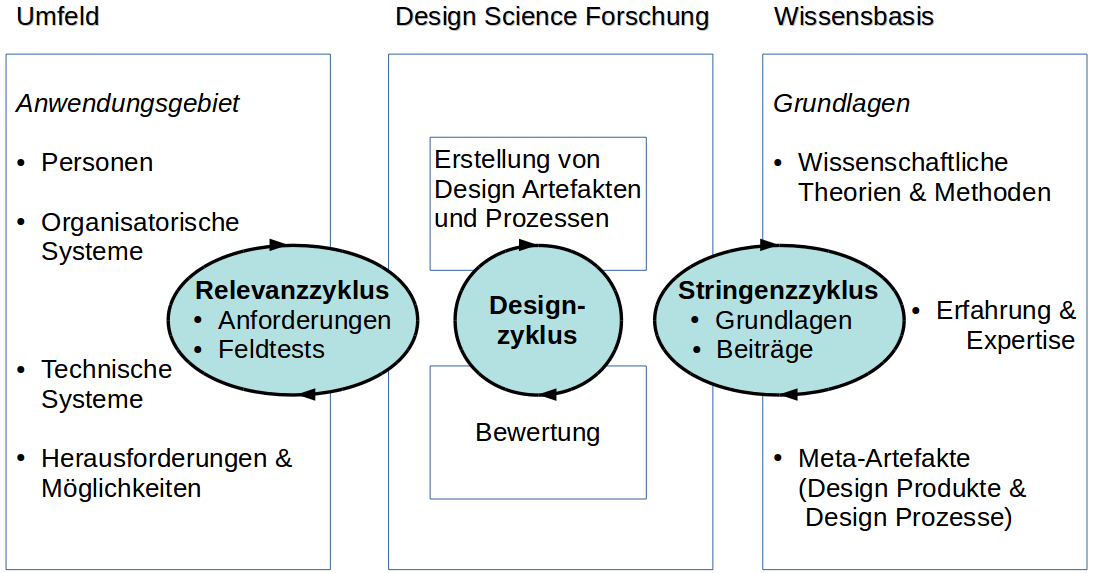
\includegraphics[scale=.3]{Drei_Zyklen_Sicht} % png ist Default für Dateiendung
\end{center}
\caption{Die drei Zyklen der Design Science Research
  \parencite[eigene Darstellung mit Übersezung in Anlehnung an][]{Hevner2007}}
\end{figure}
%
Der \Fachbegriff{Relevanzzyklus} (engl.~\Fachbegriff{Relevance Cycle}) bildet den Anfang eines 
Design Science Forschungsprojektes. In
diesem ersten iterativen Vorgang sollen die Anforderungen sowie der
Anwendungsbereich ermittelt werden. Insbesondere gilt es hier die Akzeptanzkriterien
für das vom Forscher zu erstellende IT-Artefakt zu definieren. Das fertige IT-Artefakt
kann dann wieder in das Umfeld eingebracht werden, wo es
anhand der definierten Kriterien evaluiert und getestet wird. Je nach Testergebnis und Feedback der
Stakeholder können neue Anforderungen entstehen und zusätzliche Iterationen
notwendig sein.

Der \Fachbegriff{Designzyklus} (engl.~\Fachbegriff{Design Cycle}) bildet den zentralen Zyklus 
der \Fachbegriff{Drei-Zyklen-Sicht} (engl.~\Fachbegriff{Three-Cycle-View}; s. \abbildung{ThreeCycleView}).
Dieser Zyklus wird am häufigsten iteriert, da er die Brücke zwischen dem Umfeld, in dem
das Artefakt eingesetzt wird (Relevanzzyklus), und der Wissensbasis
(Stringenzzyklus) bildet. Die Anforderungen für das IT-Artefakt kommen aus dem
Relevanzzyklus und die Methoden zur Erstellung und Evaluierung des Artefakts aus dem
Stringenzzyklus.

Der \Fachbegriff{Stringenzzyklus} (engl.~\Fachbegriff{Rigor Cycle}) greift auf eine Wissensbasis
zu, die dem Forscher
verschiedene Methoden und Werkzeuge anbietet. Dadurch soll das Projekt
einen wissenschaftlichen Stellenwert erreichen. Der Forscher erstellt mit diesem
Methodenfundus sein IT-Artefakt im Designzyklus. Dabei soll das IT-Artefakt einen
wissenschaftlichen Beitrag zur Wissensbasis leisten, indem es dem akademischen
Publikum zugänglich wird.

Jedes Forschungsprojekt, welches gemäß dem Design Science Forschungsansatz durchgeführt wird,
bedarf einer angepassten Ausprägung desselben. Hierzu können die in \tabelle{DSResearchGuidelines}
aufgelisteten Richtlinien nach \textcite{Hevneretal2004} dienen.
%
{\small
\begin{longtable}{p{.26\textwidth}p{.33\textwidth}p{.32\textwidth}}
\toprule
\textbf{Richtlinie} & \textbf{Kurzbeschreibung} & \textbf{Erzielt durch} \\
\midrule
1: Artefakt-Design & Design Science Research muss ein realisierbares Artefakt herstellen &
Prototypische Implementierung  \\*
\midrule
2: Problemrelevanz & Technologische Lösung zu einem relevanten, betrieblichen Problem &
problemspezifische Methode \\*
\midrule
3: Designbewertung & Mehrwert des Artefakts muss umfassend getestet werden & 
problemangepasster Validierungscheck  \\*
\midrule
4: Forschungsbeitrag & Verifizierbare, eindeutige Beiträge zur Forschung müssen erzielt werden &
konkreter Prototyp \\*
\midrule
5: Stringenz der\newline\phantom{5:} Forschung & Eindeutig nachvollziehbare Methoden zur
Erstellung und Evaluation des Artefakts & angewendete Forschungsmethoden  \\*
\midrule
6: Design als \newline\phantom{6:} Rechercheprozess & Suche nach einem effektiven Artefakt
erfordert Feedback und Methoden & Rücksprache mit Stakeholdern \\*
\midrule
7: Forschungs-\newline\phantom{7:} vermittlung & Design Science Research muss den Zielgruppen verständlich präsentiert werden &
strukturierte und nachvollziehbare Dokumentation \\*
\bottomrule \\
\caption{Die sieben Design Science Forschungsrichtlinien gemäß \textcite{Hevneretal2004}}
\label{tab:DSResearchGuidelines}
\end{longtable}
} % end \small
%
Dabei ist festzuhalten, dass diese Richtlinien keine feste Sequenz bilden, sondern als
voneinander unabhängig und sich ergänzend betrachtet werden können. Sie sind geeignet, den
Design Science Research Prozess zu unterstützen.

Ergänzend können bei Evaluationen oder im Relevance Cycle des Design Science Resaerch Prozesses
auch Experteninterviews eine Rolle spielen. Einer strukturierten Herangehensweise an diese widmet
sich der folgende Abschnitt.
%
\section{Interviews}
\label{sec:FM-Interviews}
%
Bei manchen Aufgaben sind strukturierte Interviews gefragt. Auch dieser Abschnitt folgt wiederum 
mit Anpassungen einer Vorversion der Bachelorarbeit von \textcite{Riedel2018}.
%

Mit dem Experteninterview als weitere Forschungsmethode können wichtige Inhalte wie
Anforderungen einer Anwendung, Zielsetzungen eines Projekts oder Probleme eines
Prozesses in einem zu untersuchenden Unternehmen festgestellt werden. Im Unterschied
zur quantitativen Umfrage erfolgt das Experteninterview qualitativ, d.h. die Aussagen
eines einzelnen interviewten Experten gelten als anerkannt und empirisch belegt
%
% mehrere Zitate in einem Befehl
%
\parencites[s.][103]{Glaeser2010}{Mayring1994}.
%
Eine genaue Definition, ab wann ein Experte als
Experte gilt, wird in der Literatur kontrovers diskutiert. Nach \textcite{Mieg2006} ist
ein Experte eine Person im Unternehmen, die mindestens 10 Jahre Erfahrung auf dem
untersuchten Gebiet hat. An anderer Stelle wird betont, dass ein Experte vor allem eine
hohe Expertise zu den befragten Themen haben sollte und die reine Erfahrungszeit nicht
maßgebend sei \parencite[s.][11 -- 12]{Glaeser2010}. Es kann daher durchaus begründet werden, 
Interviews mit Experten zu führen, die zwar nicht alle die 10 Jahres Grenze erreicht haben,
aber dennoch ein fundiertes Wissen über den Anwendungsfall besitzen.

Zur Durchführung des Interviews ist ein durchdachter Leitfaden notwendig an dem sich
das Gespräch orientiert \parencite[s.][142 -- 143]{Glaeser2010}. Dabei existieren
unterschiedliche Varianten eines Interviewleitfadens. Neben der Möglichkeit, falls vorhanden,
ein standardisiertes Leitfadeninterview zu verwenden, kann auch ein eigener Leitfaden
entwickelt werden, bei dem ein Teil der Fragen deduktiv aus der Theorie
heraus gebildet wird und ein anderer Teil der Fragen sich im Verlauf des Interviews ergibt
\parencite[s.][42]{Glaeser2010}. Eine Leitfrage soll hierbei nach \textsc{Gläser} und \textsc{Laudel}
das Wissen für ein konkretes Thema, Problem oder Forschungsfrage beschaffen. Aus
diesen Überlegungen heraus lässt sich dann ein Framework für Interviewleitfäden wie in
Tabelle \ref{tab:Interviewleitfaeden} dargestellt ableiten.

%
\begin{table}[h]
\label{tab:Interviewleitfaeden}
\begin{tabular}{llllc}
\toprule
\textbf{Leitfrage} & \textbf{Teilfrage} & \textbf{Zweck} & \textbf{Notizen} & \textbf{Ok} \\
\midrule
1. Erste Leitfrage & \parbox[c][10ex]{0pt}{} 1.1 Teilfrage & -- erwartete Antwort & & \\
\cmidrule{2-3}
                 & \parbox[c][10ex]{0pt}{} 1.2 \emph{Schlüsselfrage} & -- Ziel der Frage & (optional) & \Square                 \\ \cmidrule{2-3}
& \parbox[c][10ex]{0pt}{} 1.3 Teilfrage & \ldots & & \\
\midrule
2. Zweite Leitfrage & \parbox[c][10ex]{0pt}{} 2.1 Teilfrage & \ldots & (optional) & \Square \\
\bottomrule\\
\end{tabular}
\caption{Framework für Interviewleitfäden}
\end{table}
%
Es zeigt eine Unterteilung der Leitfragen in
Teilfragen, die die
übergeordnete Frage umfassend beantwortet. Schlüsselteilfragen sind hierbei Fragen, die
vom Interviewten in jedem Fall zu beantworten sind. Jede vordefinierte Teilfrage erzielt
einen bestimmten Output, der ebenfalls notiert werden sollte. Eine Spalte für Notizen
ermöglicht bereits während des Interviews wichtige Informationen zu notieren. Das
Framework kann als Grundlage für die Interviewleitfäden einer Arbeit dienen.
Ein Experteninterview sollte während der Durchführung aufgezeichnet werden, damit
wichtige Inhalte später noch einmal angehört werden können und eine Aufbereitung des
Gesprächsinhalts ermöglicht wird \parencite[s.][42]{Glaeser2010}. 
Nach den Interviews erfolgt die qualitative Inhaltsanalyse nach
\textcite{Mayring2010}. 

Die Auswertungsmethode sieht dabei zwei mögliche Vorgehensweisen vor:
%
\begin{compactenum}
\item die explizierende Transkription bei der das komplette Gespräch transkribiert wird und
\item die zusammenfassende Inhaltsanalyse bei der nur die inhaltsrelevanten Aussagen transkribiert werden.
\end{compactenum}
%
Meist ist Letzteres praktikabel. Zur Auswertung werden außerdem einzelne zentrale
Aussagen zu deduktiv oder zu induktiv gebildeten Kategorien zugeordnet \parencite[s.][]{Mayring2010}.
Dadurch wird eine Übersicht über die zentralen Aspekte des Interviews ermöglicht. Abbildung 
\ref{fig:Interviewkategorien} zeigt den Unterschied beider Kategorienbildungen.
%
\begin{figure}[H]
\label{fig:Interviewkategorien}
\begin{center}
\includegraphics[scale=.4]{Kategorien_Mayring}
\end{center}
\caption{Kategorienbildung induktiv (links) und deduktiv (rechts) \parencite[eigene Darstellung nach][]{Mayring1994}}
\end{figure}
%
Aus Abbildung \ref{fig:Interviewkategorien} lässt sich ableiten, dass die Kategorien bei der
induktiven Bildung anhand des Ausgangsmaterials, dem Interview, gebildet werden und bei der
deduktiven Variante die Bildung der Kategorien durch vorausgegangene theoretische
Überlegungen erfolgt. Auf eine formale Reliabilitätsprüfung sowie auf einen Kodierleitfaden
wird der Einfachheit halber verzichtet.
Mit Experteninterviews und der zusammenfassenden Inhaltsanalyse werden die
Anforderungen der neuen Anwendungslösung im untersuchten Unternehmen empirisch
erhoben und somit eine prototypische Umsetzung (bei einem Design Science Forschungsprojekt)
oder eine Auswahl zwischen Alternativen (bei Evaluationen)
gemäß dieser Kriterien ermöglicht.
%
\section{Data Science Vorgehensmodelle}
\label{sec:FM-DataScienceVorgehen}
%
Für Abschlussarbeiten mit Bezug zu \emph{Data Science} empfiehlt sich die Strukturierung des
Hauptteils der Arbeit nach dem Literaturreview gemäß einem etablierten Vorgehensmodell für
Data Science Aufgaben. Hier wird zumeist auch heutzutage noch der \gls{crispdm} verwendet,
auch wenn dieser in seiner ursprünglichen Form nicht mehr ganz auf der Höhe der Zeit ist. Es
gibt den zugehörigen Guide auch seit längerem nur noch über das \emph{Internet Archive} zu
beziehen \parencite[s.~][]{Chapman1999}.

Mittlerweile gibt es verschiedene Weiterentwicklungen von CRISP-DM, die versuchen, sowohl technischen
Neuerungen wie Cloud Computing oder Big Data aber auch modernen Ansätzen wie agilem
Projektmanagement Rechnung zu tragen. Dazu gehört auch der \Fachbegriff{Team Data Science Prozess}
von \textcite{Microsoft2018}. Die Phasen 2 -- 4 dieses Prozesses, also \emph{Datenerfassung und -auswertung},
\emph{Modellierung} und \emph{Bereitstellung} eignen sich zumeist auch gut für die Strukturierung des
Hauptteils einer Abschlussarbeit mit einer Aufgabenstellung aus dem Bereich Data Science. Daher
ist dieser Prozess als Leitlinie sowohl für die Umsetzung als auch für das Schreiben der Abschlussarbeit
bei derartigen Projekten gut geeignet.

Nach der Darstellung etablierter Forschungsmethoden für praktische Aufgabenstellungen in
Abschlussarbeiten geht es im folgenden Kapitel um 
%
\todo[color=red!40, size=\tiny]{Überleitung fertig formulieren!}
%ein weiteres essenziell wichtiges Thema bei
%der Erstellung von Abschlussarbeiten, nämlich um das Zitieren.